% This is samplepaper.tex, a sample chapter demonstrating the
% LLNCS macro package for Springer Computer Science proceedings;
% Version 2.20 of 2017/10/04
%
\documentclass[runningheads]{llncs}
%
\usepackage{graphicx}
% Used for displaying a sample figure. If possible, figure files should
% be included in EPS format.
\usepackage{gensymb}
\usepackage{url}
\usepackage{amssymb}

%
% If you use the hyperref package, please uncomment the following line
% to display URLs in blue roman font according to Springer's eBook style:
% \renewcommand\UrlFont{\color{blue}\rmfamily}

%for comments
%\newcommand{\FIXME}[1]{\textcolor{red}{FIXME: #1}}
\newcommand{\FIXME}[1]{{FIXME: #1}}

\begin{document}
%
\title{Computers Interacting with the Physical World: A First-Year Course}
%
\titlerunning{Computers Interacting with the Physical World}
% If the paper title is too long for the running head, you can set
% an abbreviated paper title here
%
\author{Roger D. Chamberlain%\orcidID{0000-0002-7207-6106}
\and
Ron K. Cytron%\orcidID{1111-2222-3333-4444}
\and
Doug Shook%\orcidID{2222--3333-4444-5555}
\and
Bill Siever%\orcidID{0000-4444-5555-6666}
}
%
\authorrunning{R.D. Chamberlain et al.}
% First names are abbreviated in the running head.
% If there are more than two authors, 'et al.' is used.
%
\institute{Dept. of Computer Science and Engineering\\
Washington University in St. Louis, St. Louis, Missouri, USA\\
\email{\{roger,cytron,dshook,bsiever\}@wustl.edu}}
%

\maketitle              % typeset the header of the contribution
%
\begin{abstract}
Most introductory embedded systems offerings are upper-division courses, aimed at juniors and seniors.  At Washington University in St.~Louis, principles of embedded systems are introduced in a first-year course that is a required for both computer scientists and computer engineers and currently has enrollments of 120-180 students each semester that it's offered. This paper describes the motivation for the course, its content, the pedagogical technique used, and lessons learned while developing and administering the course.

\FIXME{Check enrollment numbers to confirm/revise the above}

Most introductory embedded systems offerings are upper-division courses,
aimed at juniors and seniors.  At Washington University in St.~Louis, we
introduce the notion that computers interact with the physical world
in a first-year course that is a required part of the
curriculum for both computer scientists and computer engineers.
We describe the contents of the course, how it is taught, and
the lessons we have learned during its development and multiple
offerings.

\keywords{Introductory course  \and Cyber-physical systems.}
\end{abstract}
%
%
%

\section{Introduction}
\label{sec:intro}

In the spring of 2015, the Dept.~of Computer Science and Engineering at
Washington University in St.~Louis decided to make a significant change
in its first year course sequence for both computer science and
computer engineering majors.  While the first course follows, reasonably
closely, the CS1 curriculum from the ACM/IEEE~\cite{cs13}, our second semester
first-year course had a focus on thread-based parallelism.  The faculty
had collectively decided that the material in that course should be moved
to a later year (it is now offered as a sophomore-level technical elective),
and that a new course should be developed with a focus on how computers
interact with the physical world.
The new course was offered concurrently with the previous course in the
fall of 2015, and has been offered every semester since.

This paper describes that course: what we teach, how we teach it, and
what we have learned in the process.
\FIXME{Describe the highlights, including the core intellectual material,
the Arduino execution platform (which has a big hobbiest community),
the fact that it is studio-based, and a mention of the text~\cite{cc17},
contrasting with educational material with a hobbiest bent.}

The resulting course is well suited to the (admittedly differing) needs of
both computer science and computer
engineering students (e.g., we believe it is helping students discover
that they want to be computer engineers when they come into the course
not really knowing what computer engineering is).
In addition, we believe it is well positioned as an important course for
any student who wishes to be well educated in cyber-physical systems,
independent of major.
The subject matter is central to the National Academies' report on
cyber-physical systems education~\cite{nasem16}.

Unlike many introductory courses on embedded systems, which are upper-division
courses typically taken during the junior or senior year, this course is
designed to be a first-year course, accessible to students in their
first year. With the proliferation of
computing well beyond the desktop and the server room, the sheer numbers
of computers that interact with the physical world are growing and
will continue to grow.
We believe that an early (first-year) introduction to the core concepts
introduced in this course is well deserved.

The organization of the paper is as follows.  Section~\ref{sec:topics}
articulates the intellectial material that we hope to impart on the
students.  
Section~\ref{sec:delivery} describes the educational approach used,
which is a member of the active learning family.
Section~\ref{sec:weeks} provides a brief syllabus, and
Section~\ref{sec:lessons} describes what we have learned as the course
was developed and taught over the course of seven semesters.
Section~\ref{sec:conclude} concludes and describes ideas we intend
to incorporate into future offerints of the course.

\section{Intellectual Content}
\label{sec:topics}

While the course is aimed at first-year students, it is not intended to be a survey course.  It provides both exposure to and mastery of a variety of concepts in embedded and CPS, which are also significant components of the ACM's Computer Science and Computer Engineering curriculums \cite{cs13, ce16}.  Below we describe what intellectual topics we cover in the course.  Items marked with an astrisk ($^*$)   indicate topics that students are expected to have significant mastery of while non-marked items indicate concepts with lesser depth.

\subsection{Information Representation}
\label{sec:ip}
\begin{itemize}
  \item Integer Representations: Both unsigned$^*$ and Twos compliment$^*$
  \item Hexadecimal and binary representations$^*$
  \item Non-Integer Numbers: Fixed point and IEEE-754 Floating Point
  \item Character Representations: ASCII$^*$ and Unicode
  \item Character strings, both as objects and as null-terminated C-style strings
  \item Use of fields in binary representations (as in Floating Point)
  \item Bitwise operations$^*$
  \item Arrays and memory organization
  \item Representation of real-world values as voltages that require conversion to a more appropriate unit (e.g., voltage to a temperature)$^*$
\end{itemize}

\subsection{Finite-State Machines}
\label{sec:fsm}
\begin{itemize}
\item Moore style finite state machines$^*$ are a fundamental component of multiple assignments.
\end{itemize}

\subsection{Timing and Events}
\label{sec:time}
\begin{itemize}
  \item Using delays in execution (or sleep) to control time-based behavior of devices$^*$
  \item Using delta timing techniques to maintain either a fixed period between actions or fixed rate of actions (assuming a feasible schedule)$^*$
  \item Using time-division multiplexing of a shared signal line
  \item The basic structure of an event loop for event-driven programming$^*$
\end{itemize}

\subsection{Physical I/O and Circuits Principles}
\label{sec:pio}
\begin{itemize}
  \item Physical buttons and the concept of ``bounce'' on real digital inputs$^*$
  \item Analog voltages and digitization of voltages (ADC)
  \item Pulse Width Modulation
  \item Ohm's Law and current constraints/current limiting$^*$
  \item Challenges of noisy data (e.g., step detection in accelerometer data)$^*$
  \item
\end{itemize}

\subsection{Communications}
\label{sec:comm}
\begin{itemize}
  \item Serial data exchanges$^*$
  \item Non-blocking communication$^*$
  \item Byte-ordering concerns when exchanging multi-byte entities$^*$
  \item Basic protocols and the exchange of tagged records$^*$
\end{itemize}

\subsection{Architecture / Assembly Language}
\label{sec:arch}
\begin{itemize}
  \item Assembly language for integer arithmatic$^*$
  \item Registers and register conventions$^*$
  \item Function call/use protocols$^*$
  \item Stack use conventions$^*$
  \item Memory organization$^*$
  \item C-style memory segmentation (Stack, Heap, and Text segments)
\end{itemize}

\section{Instructional Delivery}
\label{sec:delivery}

\subsection{Active Learning}

For the last decade, the department has had a strong commitment to
active learning~\cite{scbggg10}.
Evidence for the benefits of active learning is
extensive~\cite{Prince04}, %jjs98,lst99,rss97
and while actively learning is applied broadly, it is particularly
compelling in science, math, and engineering
design~\cite{Freeman14},  %kb06,Byerley01,Hake98
including computer science~\cite{ag13}, %skltc10,McConnell96,tlb01
computer engineering~\cite{sr02}, %hmdpa04
and cyber-physical systems~\cite{me14}. %mmy16

While active learning is often associated with a \emph{flipped} classroom, %in
%which students work on problems during time that would otherwise be
%relegated to lecture.  A significant problem with the flipped classroom is
%that students make progress on posed problems at different
%rates.
the active learning approach we use across the entire
first year is \emph{studio}-based~\cite{hnc08}.
Our studio sessions evolved from observation of our colleagues in
Art and Architecture as they work with their students.
%As elaborated below,
%elements present in
%these sessions include collaboration, continual feedback about product
%and process, groups of 2-4 students who work at a similar rate, 
%and a problem to be solved by that group that lacks a unique
%answer or approach.  The sessions are guided but unscripted, with the
%students in a given group progressing at their own pace.

Collaboration is important for the following reasons.
Studies~\cite{Krause:2012:EFL:2157136.2157192} have shown that women are
attracted in greater numbers to the study of computer science when they
appreciate the extent to which it is practiced collaboratively.  Because
the field is largely collaborative,
featuring collaboration
in our early courses provides a more accurate impression of professional
practice to all of our students. 
%We therefore have intentionally collaborative
%sessions that allow our students to enjoy learning by interacting with others
%and to develop the skills that are useful for working in groups.

Continual feedback during studio sessions is important to keep groups on
track and to reinforce that the material is important to
their studies.  For our courses, the feedback and guidance is provided by
teaching assistants (TA) and by faculty who 
roam between the groups.  The TAs are close in age to the students in the
course.
Studies have shown that novices are more likely to predict the difficulty
of a task for other novices than are experts~\cite{Hinds:1999}.  Moreover,
the TA is more likely to empathize with the difficulty of a task than is
an expert.
%, and students appreciate the guidance of our TAs as well as their
%empathy with the difficulty of studies in computer science.

%The studio groups are arranged by the students themselves, often determined
%by the way students seat themselves in the room. In our experience, a group
%functions best when its members are closest in ability, knowledge, and
%experience.  An opposite approach would form a team with some students who
%are capable enough to help the other students in the team.  We have found
%that resentment develops by all members in such situations, so we hope for
%teams with students at the same level.   We do not take steps directly to
%form such teams.  Instead, we encourage students to move between teams in
%the first few sessions, and they usually settle in a team that is comfortable
%for them.  Another important aspect of team work in studio is that we neither
%insist upon nor do we expect that teams should reach the end of all the work
%we assign in studio.  The idea is to plow deep, not far, and we grade
%students' studio sessions on participation, 
%not on reaching any particular point in the
%studio work.  We encourage students to complete the studio work they did not
%finish in the 90-minute studio session outside our watch, 
%on their own or with team members,
%as they prefer.

Finally, the types of problems we pose in studio session are purposefully
amenable to multiple solutions and approaches.  Examples from the
first semester course include designing
a flag and anthem for a fictitious country and
determining how to draw a Sierpinski triangle.
%, and throwing darts randomly at a dartboard to compute an approximation
%of $\pi$.
Examples from this course include peak detection (counting steps in
accelerometer data) and finite-state machine design for parsing
incoming messages from another processor.
Students know there is more than one way to solve any of these
problems, which liberates them from finding the \emph{right} way and
empowers them to find their \emph{own} way.
%This lack of structure can make
%the sessions challenging for our TAs, but they enjoy watching students work
%together to create solutions in studio.

\subsection{Student Assessment}

The assessment of students includes studio
participation, on-line quizzes, assignments, and three exams.
For an individual module on a typical week,
students are expected to watch the videos
and do any required reading prior to the studio session.
A pre-studio quiz (completed on-line) is used to incentivize this
requirement.  %For a Monday studio, the first quiz is due Sunday night.
These quiz questions are designed to be straightforward to answer if
they have done what was asked of them (e.g., repetition of facts,
very simple analysis).
Studio is not graded based on correct answers, but
rather participation.

The assignment for each module is started on the
following laboratory session (on Wednesday following a Monday studio)
and is due during the laboratory session one week later.
Students are provided with a rubric with the assignment instructions,
so they know how their work will be graded. These rubrics often evaluate
not just the functionality of a submission (does it work?) but also the approach
that students use (did they choose an appropriate implementation?).
%When
%students are ready to submit their assignments, they show their work
%to a TA who will complete the rubric and submit the grade for that assignment.

The second quiz is due Wednesday evening, the same day that the assignment
is due. It is also on-line, and for this quiz the questions are 
similar in content, scope, and style as those that they are likely to
experience on the exams. 

%At three points during the semester (approximately evenly spaced) there
%is a written exam.  During each of those weeks, the
%studio session is tailored to have review content, the second laboratory
%meeting during the week does not have an assignment due, and the
%exam is scheduled in the evening so that all students are taking the
%exam simultaneously.

\section{Modules}
\label{sec:weeks}

The class starts a new module each
non-exam week, completing it the following week. There are minor schedule
adjustments around the exam, but students generally have one calendar week
to complete each module's assignment.
Also, the first laboratory meeting (labeled studio 0) is used to familiarize
the students with various logistics, such as the development environment
(both Eclipse and Arduino IDEs),
%~\cite{eclipse} and Arduino IDE~\cite{arduino}),
the code repository, etc.
The modules are described below.

\emph{Information Representation} (Module A) --
How information is represented in digital systems, including binary and
hexadecimal conversions, integer
number representations (including 2's complement), as well as
ASCII and UTF text.
Introduction to the finite-state machine abstraction,
and how to implement a finite-state machine in software.
%All of the above concepts are reinforced multiple times over the course
%of the semester, mastery is definitely not expected with only one week
%of exposure.

\emph{Microcontroller Platform} (Module B) --
How to physically implement electrical
circuits, a brief introduction to electricity (a physics course is not a
prerequisite) and voltage, digital inputs and outputs, and finite-state
machine design.

\emph{Real-Time Computing} (Module C) --
Techniques for including time as a functional
element in software. Starting with delay-based timing, students progress to delta
timing (checking each loop to determine if the desired time has elapsed).
This is combined with analog inputs (including the conversion of raw A/D
input values into engineering units) and simple filtering (averaging).
%utilizing a temperature probe that provides a 10~mv/$^\circ$C response.

\emph{Communications} (Modules D,E) (2 weeks) --
This pair of modules investigates the issues inherent in using a byte stream
to communicate between two dissimilar computer systems (the Arduino using C
and the desktop PC using Java).  Students explore how
to serialize multi-byte data types, design protocols that enable synchronization
in the face of dropped bytes,
and design finite-state machine recognizers to parse incoming messages.

\emph{Multiplexing} (Module F) --
Introduction to the concept of time-division multiplexing, asking the
students to interface to and author the software to drive a 5 by 7 pixel
LED display. Real-time computing concepts are reinforced, and students
are introduced to the fundamental mechanisms involved in larger, more
sophisticated, pixed-based displays (e.g., font design, time multiplexing).

\emph{Integrative Project} (Module G) --
Design and implementation of an integrative project
that seeks to reinforce concepts that have been introduced earlier in the
semester.  A second analog sensor is made available (an accelerometer)
for the project.
Different projects have been used in different semesters, including
the development of a pedometer and a predator-prey game (using the
accelerometer to sense the tilt of the microcontroller).

\emph{Assembly Language} (Modules H,I,J) (3 weeks) --
This three week set of modules has an introduction to basic computer
architecture
% (what is a fetch-execute engine)
and machine language, and then
focuses on assembly language, using the simple, 8-bit instruction set.
Week~1 covers data representation (especially multi-byte
data) and data manipulation
(e.g., understanding the need for a carry bit).
Week~2 introduces techniques for implementing if-then-else logic
and looping structures.
Week~3 covers pointers and array access.
%At the end of these three modules, students are not expected to be
%sophisticated assembly language programmers by any means.  The motivation
%is primarily to ensure the computer science students have been exposed,
%and the computer engineering students are better prepared for the deeper
%coverage that comes later (e.g., in their computer architecture course).

The relationship between intellectual topics and individual modules is
shown in Table~\ref{tbl:topics}. The columns in the table represent
modules, and the rows represent topics.
There is some overlap between topic names and module labels; however, that
typically implies that the specific topic is central to the module of the
same name, not that it is the only topic present in the module.

\begin{table}[t]
\caption{Relationship between intellectual topics and modules.}
\label{tbl:topics}

\centerline{\mbox{\ }\hspace{2in} Time $\longrightarrow$}
\centering
\begin{tabular}{l | c | c | c | c | c | c | c}
Topic $\Downarrow$ \ \ \ \ \ \ \ \ \ \ \ \ \ \ \ \ \ \ Module $\Rightarrow$ & A & B & C & D,E & F & G & H,I,J \\ \hline
Information Representation (\textsection 2.1) & $\blacksquare$ & $\blacksquare$ & $\blacksquare$ & $\blacksquare$ & & $\blacksquare$ & $\blacksquare$ \\ \hline
Automata (\textsection 2.2) & $\blacksquare$ & $\blacksquare$ & & $\blacksquare$ & & $\blacksquare$ & \\ \hline
Timing (\textsection 2.3) & & $\blacksquare$ & $\blacksquare$ & & $\blacksquare$ & $\blacksquare$ & \\ \hline
Circuits \& I/O (\textsection 2.4) & & $\blacksquare$ & $\blacksquare$ & $\blacksquare$ & $\blacksquare$ & $\blacksquare$ & \\ \hline
Communications (\textsection 2.5) & & & & $\blacksquare$ & & $\blacksquare$ & \\ \hline
Architecture / Assembly Lang. (\textsection 2.6) & & & & & & & $\blacksquare$ \\
\end{tabular}
%\centerline{\mbox{\ }}
%\centerline{Column Legend}
%\centering
%\begin{tabular}{c | l || c | l}
%Module & Name & Module & Name \\ \hline
%A & Information Representation & F & Multiplexing \\
%B & Microcontroller Platform & G & Integrative Project \\
%C & Real-Time Computing & H,I,J & Assembly Language \\
%D,E & Communications \\
%\end{tabular}
\end{table}

In addition to the modules described above, there are a few modules that
have been developed and used in previous semesters, but are not in current use.

\emph{Interrupts} --
Students explore how interrupts literally interrupt currently executing code.  In addition, students see how interrupts improve responsiveness to events, like button presses (which can further exacerbate bouncing).

\emph{IP Networking} --
This module introduces students to topics in networking.  IP protocols,
including both TCP/IP and UDP/IP are covered, as well as domain name service
and socket-based communications.

\section{Lessons Learned}
\label{sec:lessons}

\FIXME{What are the lessons we have learned?}

\subsection{Pacing of Material}

\FIXME{Assignments with a duration of only one week.}

As recently as the spring semester of 2017, the pacing of material
was uneven and somewhat too fast.  The following are quotes from
end-of-semester student evaluations.
\begin{itemize}
\item ``The pace was inconsistent.''
\item ``It moved a little too fast in parts and wasn't always as
in-depth as I would've liked.''
\item ``We moved pretty quickly through material and I never felt like I had
time to fully grasp concepts because the assignments took so much time.''
\item ``The class moved too quickly.''
\item ``Assignments were too long for such short period of time.''
\end{itemize}
In reaction to these comments, we've evolved the course into the organization
that is described in Section~\ref{sec:weeks}.
For example, the networking module was (at least temporarily) retired
and the assembly language material was given more time (converted from a
2 week series into a 3 week series, without expanding the content).

In the most recent semester's student evaluations (spring 2018),
the results of the pace ratings are shown in Figure~\ref{fig:pace}
(using a 7-item Likert scale).
The mean score of 5.47 is very close to the department's average of
5.66, and a substantial improvement from the mean score of 4.51
for the course in spring of 2017.

\begin{figure}[ht]
\centering
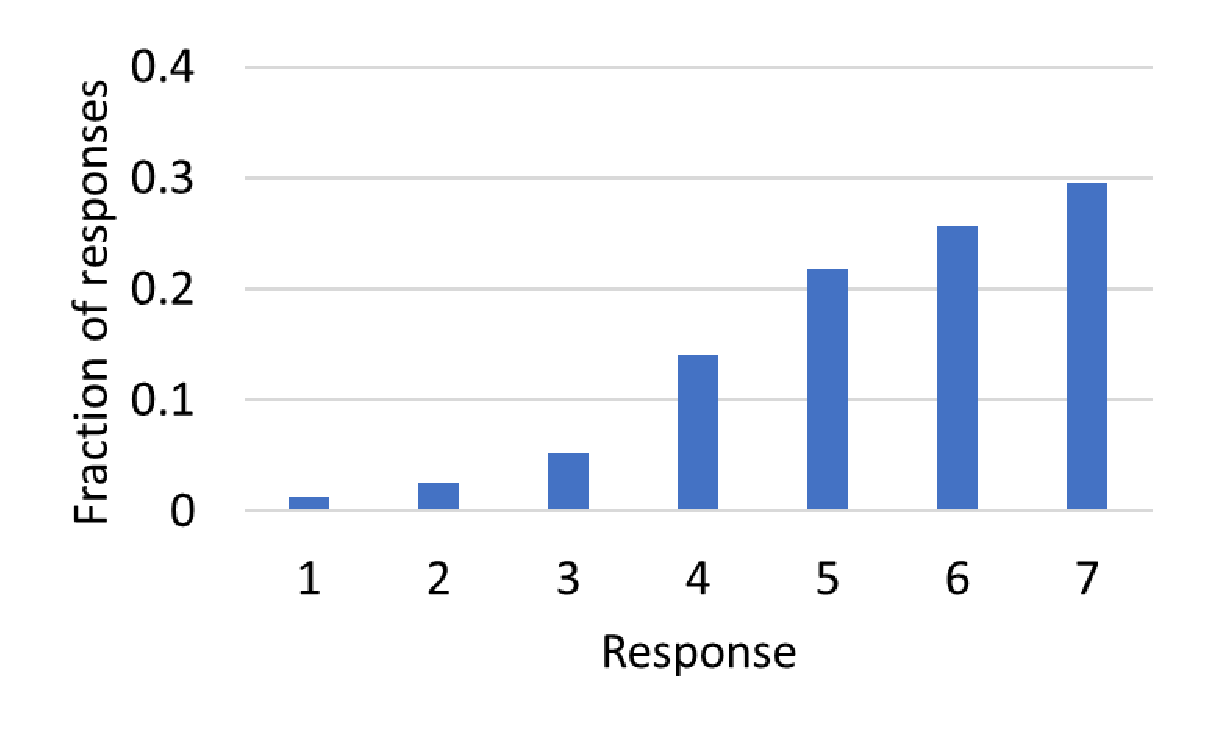
\includegraphics[width=\columnwidth]{pace}
\caption{Student ratings of statement, ``The material was covered
at a reasonable pace''  (scoring: 1 - Strongly Disagree, 7 - Strongly Agree).}
\label{fig:pace}
\end{figure}

\subsection{Analysis Problems}

Based on commentary in the literature that posits the benefits of
analysis problems in the context of design courses~\cite{wjbo01},
we were concerned that the present
course doesn't have sufficient analysis content (i.e., the bulk of
studio questions and assignment questions are design questions rather
than analysis questions).

To test this theory, we generated an additional set of analysis problems,
designed to be helpful in preparing students for the third exam, and
made them available to students one week prior to the exam.  To provide
an incentive for the students to attempt them, students were told that
there would be a small amount of extra credit for those that did well.

We then compared scores for the two groups of students, those who did
attempt the extra credit exercise and those who did not.  The results
of this comparison are shown in Figure~\ref{fig:scores}.
There clearly is a correlation between overall course grade and
whether or not a student attempted the extra exercise.
Those who attemped the extra exercise scored over 4\% higher overall
(the scores presented exclude the extra credit provided from the
exercise).  This is statistically significant at $p = 0.02$ (non-paired data).

\begin{figure}[ht]
\centering
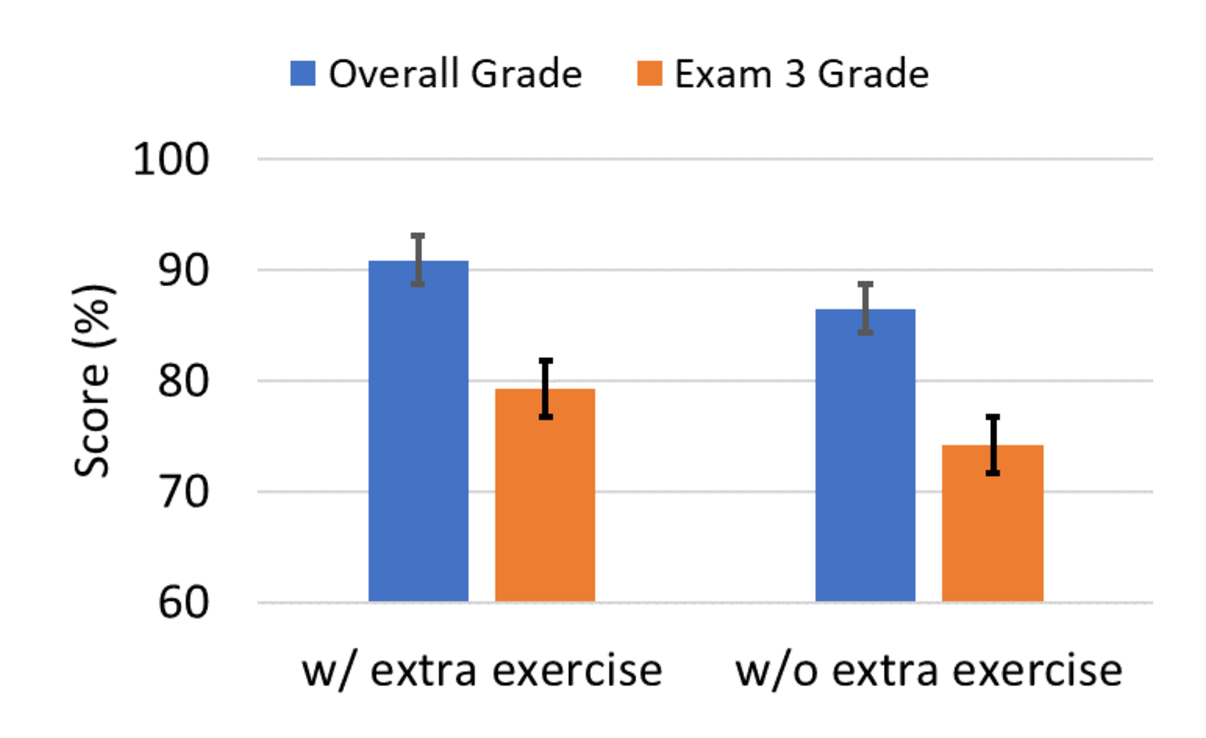
\includegraphics[width=\columnwidth]{scores}
\caption{Relationship between overall scores and exam~3 scores
with and without the extra exercise. The bars indicate mean score and
the whiskers indicate standard error.}
\label{fig:scores}
\end{figure}

When we examine the scores on exam~3, however, the story is different.
While the mean score differential is similar (at 5\% in this case), the
variability in scores is wide enough that this result is not
statistically significant ($p = 0.11$, non-paired data), so we cannot
rule out the null hypothesis that the difference in the means is
due to chance.

Our current opinion is that the correlation seen in the overall scores
is nothing as specific as a single exercise, but is more likely due to the
fact that better students (more likely to achieve a higher score prior
to the availability of an optional exercise) are also more likely than
their peers to take advantage of an optional exercise, especially when
it provides extra credit.

Going forward, we are still interested in whether or not additional
analysis problems can help students learn the material better, and will
likely pursue it by altering the mix of analysis vs.~design problems
within the studio exercises.

\subsection{Logistics}

``More structure and organization, use more difficult examples when
teaching the material since the assignments were a lot harder than
the given examples.''

``It needs more organization.'' We didn't do as good a job as we should have
in communicating due dates, etc. A number of the specifics on the calendar
were filled out (made available to the students) as the semester proceeded.
In retrospect, this was a mistake, as a number of things didn't make it on
to the calendar early enough for everyone to see them.

\FIXME{Reintroduction of "lecture" (actually recitation).}

\section{Conclusions}
\label{sec:conclude}

\FIXME{Conclusions and future stuff we want to do.}


\section*{Acknowledgements}
The authors would like to acknowledge
the generous support of the Larsen family, which has been instrumental
in the development of this course.


%
% ---- Bibliography ----
%
% BibTeX users should specify bibliography style 'splncs04'.
% References will then be sorted and formatted in the correct style.
%
\bibliographystyle{splncs04}
\bibliography{paper}
%
\end{document}
